% gjilguid2e.tex

%\documentclass[extra,onecolumn]{gji}
\documentclass[extra,mreferee]{gji}
\usepackage{timet}
\usepackage{url}
\usepackage{amsmath}
\usepackage{graphicx}
\usepackage{color, soul}

\title[TPW Rates]
  {Rates of true polar wander in convecting planets}
\author[I. Rose and B. Buffett]
  {Ian Rose$^1$ and Bruce A. Buffett$^1$ \\
  $^1$ Department of Earth \& Planetary Science, University of California, Berkeley, CA 94720, USA.  E-mail: ian.rose@berkeley.edu
  }
\date{}
\pagerange{\pageref{firstpage}--\pageref{lastpage}}
\volume{}
\pubyear{}

\let\leqslant=\leq

%in case I want to add detail to any derivation
\newif\ifdetail
\detailfalse
%\detailtrue

\begin{document}

\label{firstpage}

\maketitle

\begin{summary}
Mass redistribution in the convecting mantle of a planet can cause perturbations in its moment of inertia tensor. 
Conservation of angular momentum dictates that these perturbations can change the direction of the rotation vector of the planet, a process known as true polar wander (TPW). 
Although the existence of TPW on Earth is well-verified, its rate and magnitude over geologic time scales remain controversial. 
Here we present scaling analyses and numerical simulations of TPW due to mantle convection over a range of parameter space relevant to planetary interiors. 
For simple rotating convection, the most important parameters are the Rayleigh number, the rotation rate, and the size of relative density fluctuations (i.e. thermal expansivity times the temperature variations). 
We identify timescales for the growth of moment of inertia perturbations due to convection and for their relaxation due to true polar wander. 
These timescales, as well as the relative sizes of convective anomalies, control the rate and magnitude of TPW.
This analysis also clarifies the nature of so called ``inertial interchange'' TPW events, and when they are likely to occur.
Finally, we discuss implications for large-scale TPW in Earth's past, which has been suggested to be important for life and climate history.
\end{summary}

\begin{keywords}
Earth rotation variations; Mantle processes; Dynamics: convection currents and mantle plumes; Planetary interiors; Numerical solutions; Paleomagnetism applied to tectonics.
\end{keywords}

\section{Introduction}
\label{sec:intro}

A rotating, quasistatic body like a planetary mantle will tend to spin about the axis of its maximum moment of inertia.
Convection in a planetary mantle continuously redistributes mass, which can change the moment of ineratia tensor, necessitating a change in the spin axis of the planet to conserve angular momentum, a process known as true polar wander (TPW).

TPW was first considered in detail by \citet{darwin1887influence}, and the theory has been subsequently developed by many \citep[e.g.][]{munk1960rotation, goldreich1969some, ricard1993polar}. 
Despite this, the ability of internal mass anomalies to drive large-scale TPW remains controversial. 
Paleomagnetic data have been interpreted to require up to $\sim 1^\circ$/Myr rates of TPW \citep{mitchell2011sutton}, but the ability of the mantle to respond at such rates has been questioned \citep{tsai2007theoretical}.

The primary uncertainties in assigning a maximum TPW rate to a convecting planet are the size of convective anomalies, which drive the rotational adjustment, and the viscosity structure of the mantle, which retards it. 
These two uncertainties are not unrelated: they are both expected to be functions of the geometric and material properties of the mantle.
As such, they do not vary independently, and first-order questions about the propensity for planets to experience TPW remain: how are rates of TPW expected to vary with the vigor of convection? 
Are other planetary bodies more or less likely than Earth to experience TPW?  And are these rates expected to vary in Earth history?

These questions suggest that an approach rooted in dimensional analysis and fluid dynamics can clarify the rates and magnitudes of TPW.
Most previous studies coupling mantle convection models to polar wander calculations have done so with prescribed density perturbations \citep[e.g.][]{greff2004upwelling}, or prescribed moment if inertia variations \citep[e.g.][]{tsai2007theoretical, creveling2012mechanisms}. 
\citet{richards1999polar} coupled thermal convection models to a polar wander model, but did not address in detail the scaling relationships between the two.

Herein we perform a scaling analysis of rates of TPW for a minimal system of a rotating, convecting mantle.
We support our analysis with numerical simulations of 2D mantle convection using the finite element code \texttt{Aspect} \citep{kronbichler2012high}, based on the \texttt{deal.II} library \citep{dealII81}.  
\texttt{Aspect} provides modern numerical methods, flexible geometry, and powerful support for integrating user-defined modules and postprocessors.

\section{Rotational dynamics}

\subsection{The Liouville equation}
Conservation of angular momentum for a torque-free system in a rotating reference frame requires

\begin{equation}
\frac{d {\bf H}}{dt} + {\bf \Omega} \times {\bf H} = 0
\label{eq:euler}
\end{equation}

known as Euler's equations, where ${\bf H} = {\bf I} \cdot {\bf \Omega}$ is the angular momentum vector, $\bf I$ is the moment of inertia tensor, and $\bf \Omega$ is the angular velocity.
On a dynamic planet $\bf I$ may be a function of time, so to conserve angular momentum $\bf \Omega$ must be also vary with time.
In this case Equation \eqref{eq:euler} is known as the Liouville equation \citep[e.g.][]{munk1960rotation}.
For a slowly convecting fluid such as a planetary mantle the inertial term $\partial {\bf H} / \partial t$ is negligible, so we may solve the simplified quasistatic equations
\begin{equation}
{\bf \Omega } (t)\times ( {\bf I}(t) \cdot {\bf \Omega }(t) ) = 0
\label{eq:quasistatic_liouville}
\end{equation}

Note that solving Equation \eqref{eq:quasistatic_liouville} is equivalent to solving an eigenvalue problem for ${\bf I}$, where the eigenvectors correspond to the principal axes and the eigenvalues correspond to the principal moments (where the most stable orientation of the planet corresponds to rotating about the largest principal axis).
In practice this eigenvalue approach has been often used in previous studies for computing the spin axis of a planet \citep[e.g.][]{steinberger1997changes, roberts2007cause}.
The moment of inertia tensor in \eqref{eq:quasistatic_liouville} includes all contributions to the mass structure
of the planet, including the spherically symmetric mass distribution, rotational deformation, deformation due to self gravity, internal and surface density anomalies, and surface deflections due to density anomalies.
Here we are interested in the moment of inertia due to mantle convection, and thus neglect the contributions of surface
density anomalies (though these can be quite important, \hl{ citations for Glaciers, Tharsis, etc} ).

For mantle convection problems the moment of inertia tensor is commonly separated into three parts \citep{ricard1993polar}:

\begin{equation}
I_{ij}(t) = I_0 \delta_{ij} + J_{ij}(t) + E_{ij}(t)
\label{eq:separation}
\end{equation}

where $I_0$ is the spherically symmetric reference moment, $J_{ij}$ is the contribution due to rotational deformation, and $E_{ij}$ is the contribution due to internal density anomalies, as well as the surface deflections caused by them.
If we plug this decomposition into Equation \eqref{eq:quasistatic_liouville} the spherically symmetric part $I_0 \delta_{ij}$ drops out, and we are left with

\begin{equation}
{\bf \Omega} \times ({\bf J} \cdot {\bf \Omega}) = -{\bf \Omega } \times ( {\bf E} \cdot {\bf \Omega} )
\label{eq:disequilibrium}
\end{equation}

This form of the quasistatic Liouville equation makes clear that the polar wander problem represents a balance between the mismatches of the convective part of the moment of inertia ($\bf E$) and the rotational deformation part of the moment of inertia ($\bf J$).
Our goal is to characterize this balance from a perspective of scaling and fluid dynamics.

\subsection{Rotational deformation}

The part of the moment of inertia due to the elastic rotational deformation is traditionally related to the degree-two part of the gravity field via MacCullagh's formula \citep{munk1960rotation}:

\begin{equation}
J_{ij} = \frac{k a^5}{3 G} \left( \Omega_i \Omega_j - \frac{1}{3} \Omega_q \Omega_q \delta_{ij} \right)
\label{eq:elastic_deformation}
\end{equation}

where $k$ is an elastic Love number, $a$ is the semimajor axis of the planet, and $G$ is the gravitational constant.
This result may be extended to a viscoelastic rheology via the viscoelastic correspondence principle \citep[e.g.][]{peltier1974impulse}:

\begin{equation}
J_{ij} = \frac{k(t) a^5}{3 G} * \left( \Omega_i \Omega_j - \frac{1}{3} \Omega_q \Omega_q \delta_{ij} \right)
\label{eq:viscoelastic_deformation}
\end{equation}

where $k$ is now a time-dependent viscoelastic Love number which is convolved with the time-dependent rotation vector.

The infinite-time limit of Equation \eqref{eq:viscoelastic_deformation} allows us to calculate the fluid limit of the Love number $k_f$:
\begin{equation}
k_f = \frac{3 G (C-A)}{\Omega^2 a^5}
\label{eq:fluid_love}
\end{equation}

where $C$ and $A$ are the polar and equatorial moments of inertia, respectively.
The infinite-time limit, however, does not allow for any disequilibrium between $J_{ij}$ and $E_{ij}$.

\citet{ricard1993polar} obtain an approximation to Equation \eqref{eq:viscoelastic_deformation} which retains its long-time behavior by entering the Laplace domain and truncating a Taylor series for $k(s)$ to first order.  
This introduces a new parameter, termed $T_1$, which can be seen as a weighted tidal relaxation time for the system.  
This simple approximation in the Laplace domain allows for an analytical transformation back into the time domain, and neglecting second order terms in $\dot{\Omega}$ we find:

\begin{equation}
J_{ij} = \frac{k_f a^5}{3 G} \left( \Omega_i \Omega_j - \frac{1}{3} \Omega_q \Omega_q \delta_{ij} \right) -
 \frac{k_f a^5 T_1}{3G} \left(\dot{\Omega}_i \Omega_j + \Omega_i \dot{\Omega}_j - \frac{2}{3} \Omega_q \dot{\Omega}_q \delta_{ij} \right)
\label{eq:rotational_deformation}
\end{equation}

The two terms of this equation have simple interpretations.  
The first term corresponds to the fluid limit of rotational deformation (in the absence of any long-term elastic strength).  
The second term represents the lag in the moment of inertia due to the viscous adjustment of the rotational bulge, where $T_1$ is the characteristic time constant for this adjustment.
Since the first term represents the fluid limit of rotational deformation, it automatically satisfies Equation \eqref{eq:quasistatic_liouville}, and hence does not contribute to the polar wander problem.

\subsection{The convective moment of inertia}
\label{sec:convective_moment}

The term on the right-hand side of equation \eqref{eq:disequilibrium} represents the moment of inertia due to internal density anomalies as well as the surface deflections due to them.
This, as well, may be parameterized using a viscoelastic Love number approach:
\begin{equation} 
{\bf E} = \left[ \delta(t) + k^L(t) \right] * {\bf C}
\end{equation}

where $k^L$ is an internal loading Love number representing the surface deflection due to density anomalies, and $C_{ij}$ is the moment of inertia without that response.
Frequently the simplification is made that the timescale of the surface response is quick compared to the true polar wander timescale, and we may use the fluid limit geoid kernels \citep[e.g.][]{richards1984geoid}:  
\begin{equation}
E_{ij} = (1+k^L_f) C_{ij}
\end{equation}

An alternative to the loading Love number approach to surface deflections is to calculate the surface deflections directly using mantle convection simulations with a true free surface boundary condition.

\subsection{Rate of true polar wander}

We are in a position to address the rates of true polar wander for a given convective moment $\bf E$.
A considerable simplification occurs if we neglect secular changes in the rotation rate, and just consider changes in direction of the pole ($d \Omega^2 / dt = 2 {\Omega_i} \dot{ \Omega}_i = 0$)
Substituting Equation \eqref{eq:rotational_deformation} into Equation \eqref{eq:disequilibrium} we find

\begin{equation}
\frac{k_f a^5 T_1}{3G}{\bf \Omega} \times {\bf \dot{\Omega} } = {\bf \Omega} \times \left( {\bf E \cdot \Omega} \right)
\label{eq:liouville}
\end{equation}

Introducing a unit vector $\mitbf{\omega} = {\bf \Omega}/\|{\bf \Omega} \|$ and using Equation \eqref{eq:fluid_love} for $k_f$,  we may solve this equation for ${\bf \dot{\mitbf{\omega}} }$:
\begin{equation}
 \dot{\mitbf{\omega}}  = \frac{1}{(C-A)T_1} \left[ {\bf E \cdot \mitbf{\omega}} - \left( {\bf \mitbf{\omega} \cdot E \cdot \mitbf{\omega} } \right) \mitbf{\omega} \right]
\end{equation}

Note that the quantity in brackets is similar in form to the shear stress on a plane in classical elastostatics.
If we enter the coordinate system of the convective moment of inertia $\bf E$ with principal moments $\lambda_1 \le \lambda_2 \le \lambda_3$ and define the orientation of $\mitbf{\omega}$ with colatitude $\theta$ and longitude $\phi$ we can write this in a more illuminating form (after some tedious algebra):

\ifdetail

And here is the tedious algebra.  Let the prefactors $\frac{1}{(C-A)T_1}$ be denoted by $A$, and the pole of the coordinate system ($\theta = 0$) associated with the eigenvector for $\lambda_3$.  Therefore we find that $\mitbf{\omega} = \left[ \sin{\theta} \cos{\phi} \;\; \sin{\theta} \sin{\phi} \;\; \cos{\theta} \right]^T$.  Plugging this in, we find a system of three equations, which we want to solve for $\dot{\theta}$ and $\dot{\phi}$:

\begin{equation}
\begin{aligned}
 & \cos{\theta}\cos{\phi} \dot{\theta}  - \sin{\theta}\sin{\phi} \dot{\phi} = \\
  &A \sin{\theta}\cos{\phi}\left[ \lambda_1 - \lambda_1 \sin^2{\theta}\cos^2{\phi} - \lambda_2 \sin^2{\theta}\sin^2{\phi} - \lambda_3 \cos^2{\theta} \right] \\
 &\cos{\theta}\sin{\phi} \dot{\theta}  + \sin{\theta}\cos{\phi} \dot{\phi} = \\
  &A \sin{\theta}\sin{\phi} \left[ \lambda_2 - \lambda_1 \sin^2{\theta}\cos^2{\phi} - \lambda_2 \sin^2{\theta}\sin^2{\phi} - \lambda_3 \cos^2{\theta} \right] \\
 - &\sin{\theta} \dot{\theta} = \\
  &A \cos{\theta} \left[ \lambda_3 - \lambda_1 \sin^2{\theta}\cos^2{\phi} - \lambda_2 \sin^2{\theta}\sin^2{\phi} - \lambda_3 \cos^2{\theta} \right] \\
\end{aligned}
\end{equation}

Now multiply the top equation by $\cos{\phi}$ and the second equation by $\sin{\phi}$ and add them together to get

\begin{equation}
\begin{aligned}
 & \cos{\theta}\cos^2{\phi} \dot{\theta}  - \sin{\theta}\sin{\phi} \cos{\phi} \dot{\phi} + \cos{\theta}\sin^2{\phi} \dot{\theta}  + \sin{\theta}\cos{\phi} \sin{\phi} \dot{\phi} = \\
  &A \sin{\theta}\cos^2{\phi}\left[ \lambda_1 - \lambda_1 \sin^2{\theta}\cos^2{\phi} - \lambda_2 \sin^2{\theta}\sin^2{\phi} - \lambda_3 \cos^2{\theta} \right] + \\
  &A \sin{\theta}\sin^2{\phi} \left[ \lambda_2 - \lambda_1 \sin^2{\theta}\cos^2{\phi} - \lambda_2 \sin^2{\theta}\sin^2{\phi} - \lambda_3 \cos^2{\theta} \right] \\
 & \cos{\theta}\dot{\theta} =  
   A \sin{\theta} \left[ \lambda_1 \cos^2{\phi} +  \lambda_2 \sin^2{\phi} \right] + \\
  &A \sin{\theta} \left[ - \lambda_1 \sin^2{\theta}\cos^2{\phi} - \lambda_2 \sin^2{\theta}\sin^2{\phi} - \lambda_3 \cos^2{\theta} \right] \\
\end{aligned}
\end{equation}

Now multiply the above by $\cos{\theta}$ and the third equation by $-\sin{\theta}$ and add them to get

\begin{equation}
\begin{aligned}
 & \cos^2{\theta}\dot{\theta} + \sin^2{\theta} \dot{\theta} =  
   A \sin{\theta} \cos{\theta} \left[ \lambda_1 \cos^2{\phi} +  \lambda_2 \sin^2{\phi} \right] + \\
  &A \sin{\theta} \cos{\theta} \left[ - \lambda_1 \sin^2{\theta}\cos^2{\phi} - \lambda_2 \sin^2{\theta}\sin^2{\phi} - \lambda_3 \cos^2{\theta} \right] - \\
  &A \cos{\theta} \sin{\theta} \left[ \lambda_3 - \lambda_1 \sin^2{\theta}\cos^2{\phi} - \lambda_2 \sin^2{\theta}\sin^2{\phi} - \lambda_3 \cos^2{\theta} \right] \\
\end{aligned}
\end{equation}

After a lot of cancellation, we find

\begin{equation}
\begin{aligned}
 \dot{\theta} &= A \sin{\theta} \cos{\theta} \left[ - \lambda_3 + \lambda_1 \cos^2{\phi} + \lambda_2 \sin^2{\phi} \right] \\
              &= - A \sin{\theta} \cos{\theta} \left[ (\lambda_3 - \lambda_1) \cos^2{\phi} + (\lambda_3 - \lambda_2) \sin^2{\phi} \right] \\
              &= -\frac{A}{2} \sin{2 \theta} \left[ (\lambda_3 - \lambda_1) \cos^2{\phi} + (\lambda_3 - \lambda_2) \sin^2{\phi} \right] \\
\end{aligned}
\end{equation}

Likewise we may multiply the first equation by $-\sin{\phi}$ and the second equation by $\cos{\phi}$ and add them to get

\begin{equation}
\begin{aligned}
 & \sin{\theta} \dot{\phi} = A \sin{\theta}\cos{\phi}\sin{\phi} \left( \lambda_2 - \lambda_1 \right ) \\
& \dot{\phi} = \frac{A}{2} \sin{2 \phi} (\lambda_2-\lambda_1)
\end{aligned}
\end{equation}

\else
\fi


\begin{equation}
\begin{aligned}
\dot{\theta} &= - \frac{1}{(C-A)T_1} \sin{2 \theta} \left[ (\lambda_3-\lambda_1) \cos^2{\phi} + (\lambda_3-\lambda_2) \sin^2{\phi} \right] \\
\dot{\phi} &= \;\; \frac{1}{(C-A)T_1} \sin{2 \phi} \; (\lambda_2 - \lambda_1)
\end{aligned}
\label{eq:milankovitch}
\end{equation}

Without loss of generality we may choose the coordinate system such that $\phi=0$:
\begin{equation}
\dot{\theta} = - \frac{1}{(C-A)T_1} (\lambda_3-\lambda_1) \sin{2 \theta}
\label{eq:simple_milankovitch}
\end{equation}

These equations are a version of what has been called the ``Milankovitch theorem'' \citep{munk1960rotation}.  
Written this way, it is clear that the important quantities are $\theta$ and the differences between the eigenvalues of the convective moment $\bf E$, both of which depend on the structure and dynamics of mantle convection.  
They represent, respectively, the size of convective anomalies in the moment of inertia tensor and the angular mismatch between the rotation axis and the principle axis of the convective moment.
Both $\theta$ and $\lambda_i$ depend upon the dynamics of the convecting planetary mantle.
In order to derive estimates for them, we must consider those dynamics.

\section{Internal dynamics}
\label{sec:internal}

Mantle convection and rotational dynamics of planetary bodies are usually considered separately, yet the processes are based on a common set of governing equations. 
As such, some extra care must be taken to ensure that the equations we consider are self-consistent. 
For simplicty we consider an isoviscous planet in a rotating reference frame with no internal heating in the incompressible Boussinesq approximation.  The equations for mass, momentum, and energy then read

\begin{equation}
\nabla \cdot {\bf u} = 0
\label{eq:conserve_mass}
\end{equation}

\begin{equation}
\begin{aligned}
- \nabla P + \eta \nabla^2 {\bf u} =  \rho {\bf g} -  \rho{\bf \Omega \times \Omega \times r}
\label{eq:navier_stokes}
\end{aligned}
\end{equation}

\begin{equation}
\frac{\partial T}{\partial t} + {\bf u} \cdot \nabla T = \kappa \nabla^2 T
\label{eq:energy}
\end{equation}
here the parameters are defined in Table~\ref{tab:parameters}.
In addition we use the simple equation of state
\begin{equation}
\rho = \rho_0 \left( 1 - \alpha (T-T_0) \right)
\label{eq:eos}
\end{equation}
where $\bf u$ is the velocity, $P$ is the pressure, and $T$ is the temperature.
The other parameters are defined in Table \ref{tab:parameters}.
Note that here we retain the centrifugal term, which is normally either neglected or absorbed into a modified pressure.
Dimensional analysis of this system (cf. \citet{barenblatt1996scaling}) requires four nondimensional numbers to characterize it.
Convenient choices for these numbers are listed in Table \ref{tab:nondim}, along with approximate Earth-like values for them.

In particular, the two most important numbers are the Rayleigh number, characterizing the vigor of convection, and the ratio of centrifugal to gravitational forces.
This second nondimensional number does not have a uniformly agreed-upon name, but has been called a Froude number in analogy with other applications of inertial-to-gravitational effects \citep{mckenzie1968influence}, which we adopt here.
Since we have begun with equations that do not have inertia or compressibility, we have implicitly thrown out the dependence on the nondimensional numbers which characterize those effects (e.g., the Prandtl and dissipation numbers).
It would be straightforward to include them, and they do not affect the overall treatment of this scaling.

In this case the dynamics can be characterized in terms of deviations from a reference hydrostatic state, which includes the dynamic pressure $P^* = P - P_0$ and density perturbations $\delta \rho = \rho- \rho_0 = - \rho_0 \alpha (T-T_0)$.
In addition, we expect deviations in the figure of the planet from its hydrostatic shape, which we denote by $V = V_H + \Delta V$, where $V_H$ is the hydrostatic figure and $\Delta V$ is the deviation.
The introduction of $\Delta V$ requires another nondimensional number to characterize it, and we find that the quantity $\Gamma = \alpha \Delta T$ is convenient.
Finally, we define $\mitbf{\Omega} = \Omega_0 \mitbf{\omega}$, where $\mitbf{\omega}$ is a unit vector in the direction of $\mitbf{\Omega}$.

By definition the hydrostatic reference state is a solution to \eqref{eq:navier_stokes} where there is no flow:

\begin{equation}
\begin{aligned}
- \nabla P_0 =  \rho_0 {\bf g} -  \rho_0 {\bf \Omega \times \Omega \times r}
\label{eq:hydrostatic}
\end{aligned}
\end{equation}

Nondimensionalizing with the parameters in Table \ref{tab:nondim} and removing the reference state we find the nondimensional momentum equation:
\begin{equation}
\begin{aligned}
 - \nabla P^* + \; \nabla^2{\bf v} - \mathrm{Ra} \; T \; {\bf g} + \mathrm{Ra \; Fr}\; T \;{\mitbf{\omega} \times \mitbf{\omega} \times {\bf r}} = 0
\end{aligned}
\end{equation}

Equation \eqref{eq:navier_stokes} can be transformed into an angular momentum equation by crossing with $\bf r$ and integrating over the volume of the mantle:

\begin{equation}
\begin{aligned}
-\int_V {\bf r} \times \nabla P + \int_V \eta {\bf r} \times \nabla^2 {\bf u} - \int_V \rho {\bf r \times g} + \int_V \rho {\bf r \times \mitbf{\Omega} \times \mitbf{\Omega} \times {\bf r }} &= 0 \\
\end{aligned}
\end{equation}


The first three terms represent pressure, viscous torques, and gravitational torques on the mantle.  
Convection in the outer core, atmospheres, and oceans is not strong enough to provide significant pressure and viscous torques over geologic timescales, and a self-gravitating body cannot self-torque \citep{braginsky1995equations}.
Therefore, the we can neglect those terms, and we are left with

\begin{equation}
\begin{aligned}
\int_V \rho {\bf r \times \mitbf{\Omega} \times \mitbf{\Omega} \times {\bf r }} &= 0 \\
\end{aligned}
\end{equation}

which is a statement that a quasistatic body will rotate around the principle axis of its total moment of inertia.

Splitting the volume into $V_H$ and $\Delta V$ and substituting \eqref{eq:eos} we find

\begin{equation}
\begin{aligned}
&\int_{V_H} \rho_0 {\bf r \times \mitbf{\Omega} \times \mitbf{\Omega} \times {\bf r }} + 
\int_{V_H} \rho_0 \alpha (T-T_0) {\bf r \times \mitbf{\Omega} \times \mitbf{\Omega} \times {\bf r }} +  \\
&\int_{\Delta V} \rho_0 {\bf r \times \mitbf{\Omega} \times \mitbf{\Omega} \times {\bf r }} + 
\int_{\Delta V} \rho_0 \alpha (T-T_0) {\bf r \times \mitbf{\Omega} \times \mitbf{\Omega} \times {\bf r }} = 0  \\
\end{aligned}
\end{equation}

The first term of this equation is zero due to the hydrostatic equation.  
The fourth term is negligible due to being second order in the smallness parameters $\Delta V/V_H$ and $\Gamma$.
Removing these, we find
\begin{equation}
\begin{aligned}
\int_{\Delta V} \rho_0 {\bf r \times \mitbf{\Omega} \times \mitbf{\Omega} \times {\bf r }} = 
-\int_{V_H} \rho_0 \alpha (T-T_0) {\bf r \times \mitbf{\Omega} \times \mitbf{\Omega} \times {\bf r }}
\end{aligned}
\end{equation}

This equation may be identified with \eqref{eq:disequilibrium}, where disequilibrium in the rotational deformation (left side) is balanced by the mismatch of the convective moment of intertia with the spin axis (right side).
Our goal is to identify characteristic sizes of these quantities, which must be functions of the nondimensional numbers identified in Table \ref{tab:nondim}.

\ifdetail
\subsection{Buckingham Pi theorem and nondimensionalization}
The Buckingham Pi theorem (essentially an application of the rank-nullity theorem) allows us to determine the number of nondimensional numbers for this problem.
We count the number of fundamental units for the problem, in this case mass (kg), length (m), time (s), and temperature (K), as well as the number of parameters in use for this problem.  
These parameters are listed in Table \ref{tab:parameters}, and subtracting the ...

\begin{table}
\centering
\caption{Nondimensionalizations for variables, primed variables denote dimensional variables}
\label{tab:nondim_convert}
\begin{tabular}{@{}lll}
$x^\prime$ &=& $R \;\; x$ \\
$t^\prime$ &=& $R^2/\kappa \;\; t$ \\
$T^\prime$ &=& $\Delta T \;\; T$ \\
$\rho^\prime$ &=& $\rho_0 \;\; \rho$\\
$v^\prime$ &=& $\kappa/R \;\; v$ \\
$P^\prime$ &=& $\eta \kappa/R^2 \;\; P$ \\
$\Omega^\prime$ &=& $\Omega_0 \;\; \Omega$ \\
$g^\prime$ &=& $g_0 \;\; g$
\end{tabular}
\end{table}

If we plug these nondimensionalizations into the governing equations we find that the incompressibility constraint remains unchanged.  
The temperature equation and equation of state become

\begin{equation}
\frac{\partial T}{\partial t} + {\bf v} \cdot \nabla T = \nabla^2 T
\end{equation}

\begin{equation}
\rho = 1 - \alpha \Delta T \;\;  T
\end{equation}

We may furthermore define a hydrostatic reference state where the density is the reference density everywhere and the velocity is zero, i.e.

\begin{equation}
 \rho_0{\bf \Omega \times \Omega \times r}= - \nabla P_0 + \rho_0 {\bf g}


Subtracting this from the momentum equation and defining a dynamic pressure $P^* = P - P_0$, we find

\begin{equation}
\begin{aligned}
 - & \Omega_0^2  \alpha  \Delta T T R \; {\bf \Omega \times \Omega \times r} = - \eta \kappa / R^2 \; \nabla P^* \\ 
&+ \eta \kappa / R^2 \; \nabla \cdot \left( \eta \epsilon ({\bf v}) \right) - \alpha \Delta T g_0 \; {\bf g}
\end{aligned}
\end{equation}

\begin{equation}
\begin{aligned}
 - & \mathrm{Ra \; Fr}\; T \; {\bf \Omega \times \Omega \times r} = - \nabla P^* \\ 
&+ \; \nabla \cdot \left( \eta \epsilon ({\bf v}) \right) - \mathrm{Ra} \; T \; {\bf g}
\end{aligned}
\end{equation}

  
\fi

\begin{table}
\centering
\caption{Parameters for rotating mantle convection}
\label{tab:parameters}
\begin{tabular}{@{}lcc}
Symbol & Definition\\
\hline
$R_i$ & inner radius \\
$R$ & outer radius \\
$\Omega_0$ & reference rotation rate \\
$\eta$ & viscosity \\
$\kappa$ & thermal diffusivity \\
$g_0$ & reference gravity \\
$I_0$ & reference moment of inertia \\
$T_0$ & reference temperature \\
$\delta \rho = \rho_0 \alpha \Delta T$ & buoyancy parameter \\ 
\end{tabular}
\end{table}

\begin{table}
\centering
\caption{Nondimensional numbers with approximate Earthlike values}
\label{tab:nondim}
\begin{tabular}{@{}lcccc}
Symbol &  Number & Definition & Approximate value \\
\hline
Ra & Rayleigh &  $\rho_0 g_0 \alpha \Delta T R^3/\eta \kappa$ & $10^7$\\
Fr & Froude & $\Omega_0^2 R/g_0$ & $10^{-3}$ \\
A & aspect ratio & $R_i/R$ & $0.54$ \\
$\Gamma$ & density deficit &$ \alpha \Delta T$ & $10^{-2}$ \\
\end{tabular}
\end{table}
 
\section{Scaling}
\label{sec:scaling}

It is useful to define a nondimensional eigenvalue difference (or ``eigengap'') $\Lambda_{ij} \equiv (\lambda_i - \lambda_j)/I_0$.  
This quantity represents the size of fluctuations in the convective moment of inertia compared to the reference value.
With this we may rewrite Equation \eqref{eq:simple_milankovitch} in terms of the nondimensional numbers defined above.
The difference in the polar and equatorial moments of the hydrostatic planet $(C-A)$ is proportional to the rotational to gravitational forces, or Froude number \citep{munk1960rotation}.
\begin{equation}
(C-A) \sim I_0 \mathrm{Fr}
\end{equation}

The time constant $T_1$ is a viscous tidal relaxation time of the planetary mantle. It is frequently represented as a weighted average of the different relaxation modes \citep[e.g.][]{ricard1993polar, greff2004upwelling}, but for our purposes it is enough to approximate it as a single mode:
\begin{equation}
T_1 \sim \frac{ \eta }{ \rho_0 g_0 R} = \frac{R^2}{\kappa} \frac{\Gamma}{\mathrm{Ra} }
\end{equation}
Plugging these scalings into equation \eqref{eq:simple_milankovitch} we find

\begin{equation}
\frac{\kappa}{R^2} \; \dot{\theta} \sim - \frac{\mathrm{Ra}}{\Gamma \mathrm{Fr}} \Lambda_{31} \sin{2 \theta}
\label{eq:scaled_rotation}
\end{equation}

At this point we do not have estimates for the characteristic magnitudes of $\Lambda_{ij}$ or $\theta$, both of which are crucial for predicting characteristic rates of TPW.
They represent, respectively, the size of convective anomalies in the moment of inertia tensor and the angular mismatch between the rotation axis and the principle axis of the convective moment.


The quantites $\Lambda_{ij}$ and $\theta$ should be functions of our nondimensional parameters $\mathrm{Ra}$, $\mathrm{Fr}$, and $\Gamma$.  
We consider relatively slowly rotating bodies here ($\mathrm{Fr} \ll 1$), and so make the simplifying assumption that the rotation does not significantly affect the style of convection.  
In this regime, therefore, we neglect the dependence on $\mathrm{Fr}$, and look for scalings of the form $\Lambda_{ij}(\mathrm{Ra})$ and $\theta(\mathrm{Ra})$.


\subsection{An estimate of $\Lambda_{ij}$}

\begin{figure*}
\centering
\label{fig:eigengap}
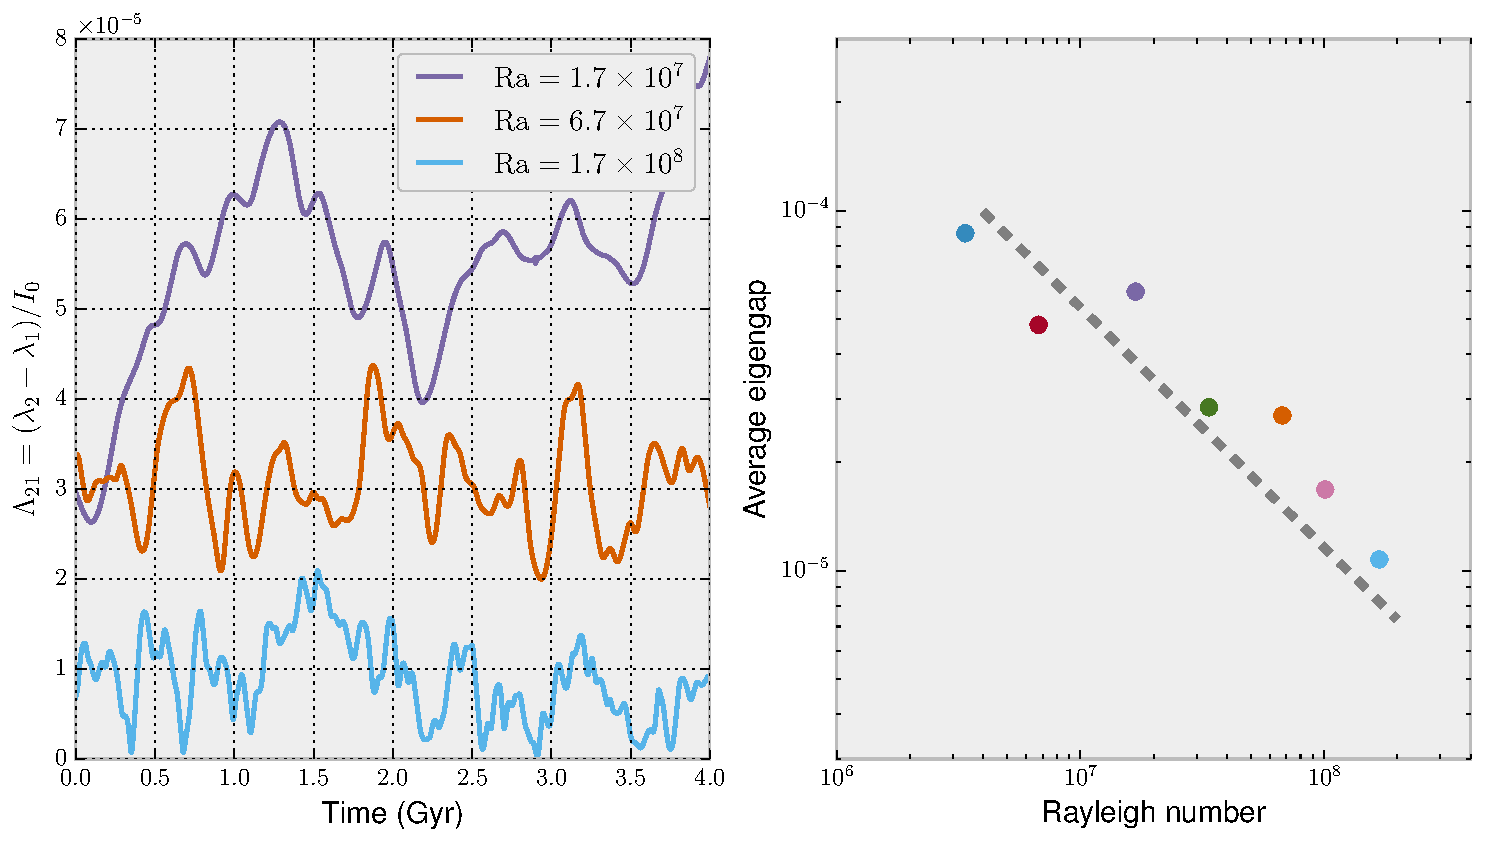
\includegraphics[width=0.9\textwidth]{figures/eigengap.pdf}
\caption{ Left: Time series of the normalized difference between moments $\Lambda_{12}$ for convection in a 2D annulus at several different Rayleigh numbers.  As the Rayleigh number increases, the average value of the relative moment decreases due to less low-degree coherence in the temperature structure.  Right:  average value of $\Lambda_{12}$ for the different Rayleigh numbers.  Also shown is a line with slope $\mathrm{Ra}^{-2/3}$, which is predicted from the scaling analysis (the exponent is $-2/3$ instead of $-1$ due to the reduced dimensionality of the simulations).}
\end{figure*}


Fluctuations in the nonhydrostatic moment of inertia are due to temperature fluctuations in the interior and their spatial structure:

\begin{equation}
C_{ij} = \int_{V_S} \rho_0 \alpha (T-T_0) \left( r_q r_q \delta_{ij} - r_i r_j \right) dV
\label{eq:temperature_fluctuations}
\end{equation}
where $V_S$ is the reference spherical volume of the mantle.
As discussed in Section \ref{sec:convective_moment}, these internal density loads may be convolved with their surface responses to get the convective moment of inertia $E_{ij}$.
The surface response is a function of the viscosity structure of the planet and the wavelength of the interal load, but the multiplicative factor $(1+k^L_f)$ is generally an order-one parameter, so we neglect it for this scaling.

For thermal convection, the convective part of the moment of inertia $E_{ij}$ is directly related to the quadrupole structure of the temperature field (see Appendix \ref{appendix:moments}).
Therefore, an estimate of one allows an estimate of the other.
We can expand the temperature structure of the convecting planet with a set of orthonormal basis functions $R_n Y_{lm}$, 
where $Y_{lm}$ are spherical harmonics, $R_n$ are some set of orthogonal radial polynomials.  
\begin{equation} 
T( r , \theta, \phi, t )  = \Delta T {\displaystyle \sum_{n=0}^\infty \sum_{l=0}^\infty \sum_{m=-l}^{l} } T_{lmn}(t) R_n(r) Y_{lm} (\theta , \phi)
\label{eq:T_series}
\end{equation}
Where the $T_{nlm}$ are the coefficents for the expansion which have been normalized by $\Delta T$.

The integral in Equation \eqref{eq:temperature_fluctuations} is picking out a degree-two spherical harmonic in the lateral dimensions, and a degree-two polynomial in radius.
We therefore want to estimate the power in a single mode of the temperature expansion, allowing us identify
\begin{equation}
\Lambda_{12} \sim \Gamma T_{202}
\end{equation}

The temperature field has been normalized by $\Delta T$ and thus goes between zero and one, therefore the expansion in $T_{lmn}$ is constrained by

\begin{equation}
\lVert T(x,y,z, t) \rVert_\infty = \lVert {\displaystyle \sum_{n=0}^\infty \sum_{l=0}^\infty \sum_{m=-l}^{l} } T_{lmn}(t) R_n(r) Y_{lm} (\theta , \phi) \rVert_\infty = 1
\end{equation}

This is a strong constraint, but it gives very little information about the distribution of power across the $T_{lmn}$.  
We can, however, think about the power spectrum in two different regimes: that of steady/quasisteady flow (relatively low $\mathrm{Ra}$) and that of chaotic flow (relatively high $\mathrm{Ra}$).
The structure of thermal convection is primarily controlled by the Rayleigh number.  Once the Rayleigh number is sufficiently high ($\sim10^6$) 
the style of convection changes from steady/quasisteady to chaotic.  Accompanying this transition to chaos is a broadening of the spatial 
and temporal spectra \citep{mclaughlin1982transition}.  

At low Rayleigh number we expect the spectrum of the temperature field to be dominated by only a few low-degree modes which are largely influenced by the aspect ratio.
This spectrum may or may not have a lot of power in degree-two, does not depend strongly on time.

At high Rayleigh number we expect the shortest lengthscales to be limited by the effects of thermal diffusion,
which tends to wipe out thermal heterogeneity at small scales.  Consequently, there will be no power in modes
with shorter lenghtscales than that allowed by diffusion. 
Therefore we expect, to a good approximation, that the infinite sum in Equation \eqref{eq:T_series} can be truncated at some maximum wavenumber, set by the smallest lengthscale $d$:
\begin{equation}
n_{\mathrm{max}}, l_{\mathrm{max}}, m_{\mathrm{max}} \sim \frac{R}{d}
\end{equation}
The total number of modes that are accessible to the system are therefore 

\begin{equation}
N_{\mathrm{modes}} = n_{\mathrm{max}} \times l_{\mathrm{max}} \times m_{\mathrm{max}} \sim \left( \frac{R}{d} \right)^{3}
\end{equation}

The value of each $T_{lmn}(t)$ will in general be some complex function of time, but for a given style of convection we expect there to be some average value.
For chaotic flow the power should be spread out amongst the modes accessible to it.
We may make the hypothesis that each of the modes are roughly as likely as any of the others, which implies

\begin{equation}
T_{\mathrm{degree 2}}(t) \sim \frac{1}{N_{\mathrm{modes}}} \sim \left( \frac{d}{R}\right)^3
\end{equation}

Any of a number of scaling laws can provide an estimate for the characteristic length scale of a convecting system which may depending on rheology, geometry, or density structure.
The simplest, based on boundary layer theory \citep{turcotte1967finite}, finds $d/R \sim \mathrm{Ra}^{-1/3}$, thus furnishing us with an estimate of the power in the degree-two part of the field as a function of Rayleigh number:

\begin{equation}
T_{\mathrm{degree 2}}(t) \sim \mathrm{Ra}^{-1}
\label{eq:degree_two_of_ra}
\end{equation}
For two-dimensional simulations there is a reduced dimensionality when calculating the number of modes,
so $N_\mathrm{modes} \sim \left(R/d \right)^2$.  This leads us to a scaling of $T_{\mathrm{degree2}} \sim \mathrm{Ra}^{-2/3}$, which is used in the simulations shown in Figure~\ref{fig:eigengap}.
This result has a simple interpretation.
As the Rayleigh number of the system increases, the smallest lengthscale of convective features gets smaller.
The total power in the temperature field is spread across a larger spectrum, leaving less total power for the degree-two part, which is what drives TPW.


With an estimate for the power in the degree-two part of the temperature field, we may finally estimate $\Lambda_{ij}$:

\begin{equation}
\Lambda_{ij} \sim \frac{\Gamma}{\mathrm{Ra} }
\end{equation}

Other power spectra for the temperature field are possible. Isoviscous models tend to be ``bluer,'' and models with viscosity stratification tend to be ``redder'' \citep{richards1999polar}.
Nevertheless, at high Rayleigh number the expectation is that the power is distributed across many length scales.


\subsection{An estimate of the mismatch $\theta$}

The mismatch between the current axis and the principle axis of the convective moment is perhaps the most important parameter in Equation \eqref{eq:scaled_rotation}.  
Much of the debate around the existence and magnitude of TPW on Earth comes down to the question of how big $\theta$ can be \citep{kirschvink1997evidence, steinberger1997changes}.

An estimate for $\theta$ must concern the stability of the convective moment of inertia. 
Convection is continuously redistributing mass throughout the mantle, which will perturb the convective moment of inertia.  
If the convective moment is stable to small perturbations, then $\theta$ should be small, but if it is not stable to perturbations, then $\theta$ could be up to $90^\circ$. 
Given a random perturbation to that moment, we would like to give a bound on how big the perturbation to $\theta$ is. 
This may be done by application of a theorem due to \citet{davis1970rotation}.

Let $\delta$ be the size of the perturbation to the convective moment of inertia tensor, and let $\lambda_3 \ge \lambda_2 \ge \lambda_1$ be the eigenvalues of that tensor.  
Then the rotation of the principal axes of the tensor is bounded by

\begin{equation}
\lVert \sin(2 \theta) \rVert \le \frac{ 2 \lVert \delta \rVert}{ \displaystyle \min_{i \neq j} \lVert \lambda_i - \lambda_j \rVert }
\label{eq:kahan}
\end{equation} 

That is to say, if there is a large difference between the eigenvalues, this stabilizes axes to perturbations.  
If, however, there is a small difference between the eigenvalues (i.e., they are nearly degenerate), then perturbations can cause large rotations of the principle axes.
This is illustrated in Figure \ref{fig:perturb}


We may arrive at a simple estimate of the growth rate of the angle $\theta$ by differentiating Equation \eqref{eq:kahan}, tentatively holding $\lVert \lambda_i - \lambda_j \rVert$ fixed:

\begin{equation}
\lVert \dot{\theta} \rVert \le \frac{ \lVert \dot{\delta} \rVert}{ \displaystyle \min_{i \neq j} \lVert \lambda_i - \lambda_j \rVert }
\label{eq:grow_perturbation}
\end{equation} 

\begin{figure*}
\centering
\label{fig:perturb}
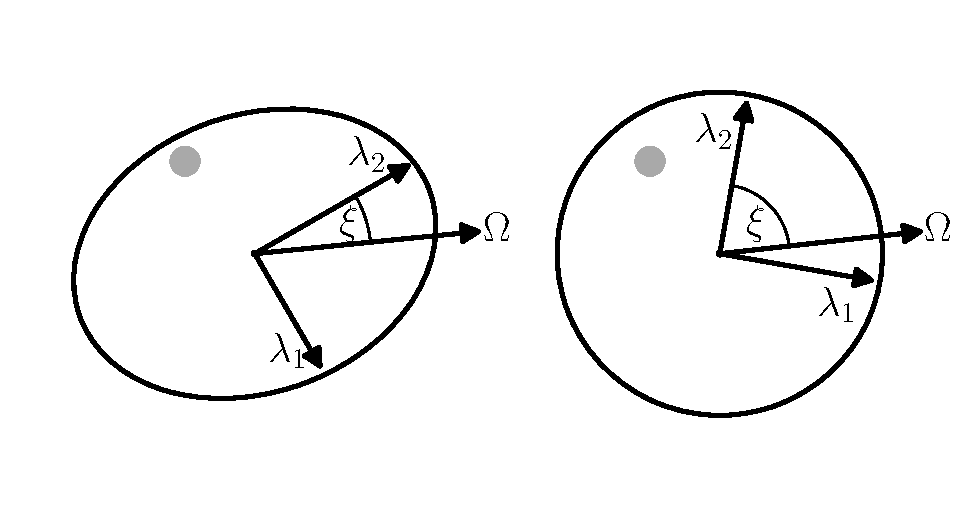
\includegraphics[width=0.9\textwidth]{figures/perturb.pdf}
\caption{Graphical demonstration of the $\sin{2 \theta}$ theorem of \citet{davis1970rotation}.  Two spheroidal bodies with eigenvalues $\lambda_2 > \lambda_1$ start out with the rotation axis $\Omega$ aligned with the $\lambda_2$ axis. However, on the left the eigengap $\lVert \lambda_2 - \lambda_1 \rVert$ is large, while on the right it is small.  A negative mass perturbation is instantaneously added to both bodies, which effects a small rotation of the principle axes on the left, but a large one on the right.}
\end{figure*}


Furthermore, the quantity $(\lambda_i-\lambda_j)$ which appears in the denominator of these equations is precisely the same as the quantity which we estimated in the previous section to scale with $\sim \mathrm{Ra}^{-1}$.
Therefore, as the Rayleigh number increases, the characteristic gap between the eigenvalues of the convective moment becomes smaller.  
Additionally, the timescale of fluctuations in these values goes down. 
Overall, this makes the principle axes of high Rayleigh number systems much less stable.
This is consistent with the result of \citet{richards1999polar}.

In the limit that the eigengap becomes zero, the rotation of the pinciple axes can be arbitrary. 
This essentially corresponds to the hypothesized ``inertial interchange true polar wander'' \citep{kirschvink1997evidence}.
We suggest, then, that a more vigorously convecting planet is much more likely to experience rapid TPW events.

\begin{figure*}
\centering
\label{fig:misfit}
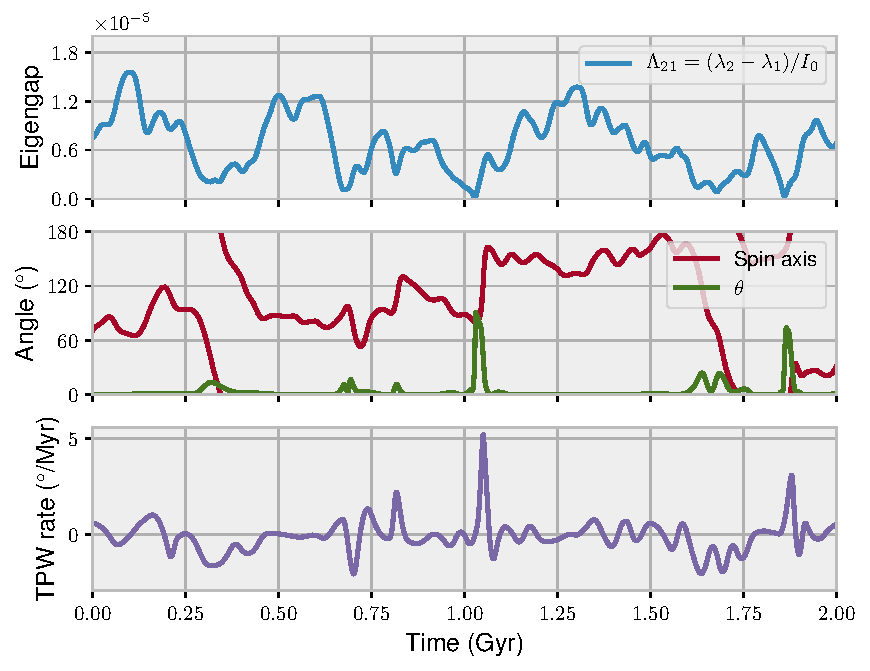
\includegraphics[width=0.9\textwidth]{figures/misfit.pdf}
\caption{Top: Time series of principle moments for 2D annular convection at $\mathrm{Ra}\sim10^8$.  Bottom: Time series of spin axis and mismatch angle $\theta$.  When the two moments are close to each other (small eigengap), the mismatch angle becomes large, and the rate of polar wander is significantly larger.}
\end{figure*}



\section{Discussion}
\label{sec:discussion}

The preceding results clarify the complex relationship between the Rayleigh number, the Froude number and the rates of TPW for a convecting planet.
As mantle convection redistributes mass in the planet's interior, the rotational bulge moves around to stay aligned with the principle axes of the convective moment of inertia. 
There is a constant competition between growth of the mismatch angle $\theta$ through Equation \eqref{eq:grow_perturbation} and its relaxation through Equation \eqref{eq:simple_milankovitch}.
We may plug in the estimate for $\Lambda_{ij}$ into equation \eqref{eq:simple_milankovitch} to find the strikingly simple expression
\begin{equation}
\frac{\kappa}{R^2} \; \dot{\theta} \sim -\frac{1}{\mathrm{Fr}} \sin{2 \theta}
\label{eq:simplest_milankovitch}
\end{equation}
Surprisingly, $\Gamma$ and $\mathrm{Ra}$ have completely dropped from the prefactor in the scaling. 
At high Rayleigh numbers response timescales for relaxation of the mismatch angle go down.
At the same time, however, coherence in the temperature structure goes down, reducing the amount of power in the degree-two part of the field responsible for driving TPW.
That these two effects cancel is something of a coincidence due to the simple estimate of the smallest lengthscales of the problem.
Scalings for lengthscales of convection in fluids with temperature dependent viscosity \citep[e.g.][]{solomatov1995scaling} or pseudoplastic rheology \citep[e.g.][]{korenaga2010scaling} have different functional dependencies on $\mathrm{Ra}$ or additional nondimensional parameters.
However, a common feature in most scalings is that typical lengthscales are still some power-law of Rayleigh number $d \propto \sim \mathrm{Ra}^{-\beta}$.
With this form, our scaling for TPW rate has the following dependence on $\mathrm{Ra}$:
\begin{equation}
\dot{\theta} \propto \mathrm{Ra}^{1-3\beta}
\end{equation}
In general, $\beta$ is some small number between one-fourth and one-third, so we expect that more complicated estimates for $d(\mathrm{Ra})$ will still show a weak dependence on the Rayleigh number.

We then suggest that the most important parameters are the Froude number, which acts as the brakes on the system, and $\theta(\mathrm{Ra})$.
Whereas the rest of the expression has at most a weak dependence on $\mathrm{Ra}$, this is expected to be strongly dependent on it.

Indeed, we can identify two endmember behaviors of Equation \eqref{eq:simplest_milankovitch}.
When convection is not sufficiently chaotic to create a large $\theta$ we are in the regime where the planet's rotation axis closely tracks that of the convective moment.
This is the regime considered in \citet{steinberger1997changes}, \citet{roberts2007cause}, and \citet{zhong2007supercontinent}, and can be considered the ``slow TPW'' regime.
When convection is more chaotic, however, there may be large excursions in $\theta$, which can drastically increase the wander rate.  
If $\theta=90^\circ$, this corresponds to IITPW \citep{kirschvink1997evidence}.  
This, however, is a special case in the large $\theta$, ``fast TPW'' regime.

As an example, we may consider the early Earth, when the mantle was presumably hotter and less viscous, leading to a 
higher Rayleigh number. We would then predict that convection was more vigorous, leading to 
a less stable $\theta(t)$, and thus more TPW and more frequent ``fast TPW'' events.

Thus far we have restricted our discussion to planets with lithospheres lacking long-term elastic strength.
For this case the long-time limit of the planetary figure is coaxial with the convective 
moment of inertia. This assumption is not necessarily true in all cases.
Earth's lithosphere is pervasively fractured and hydrated, and may not have strength on geologic timescales.
However, a planet with a stagnant lid (such as Mars) may have some strength, preventing the figure of the planet 
from reaching the fluid limit of Equation~\eqref{eq:fluid_love}.

The theory of TPW response for the case of elastic lithospheres has been developed in, among other places, 
\citet{matsuyama2006rotational}, \citet{creveling2012mechanisms}, and \citet{chan2014time}.
The formalism developed in Section~\ref{sec:scaling} can still be applied to this case, 
though the response to internal variations in the moment of inertia becomes more limited 
(and potentially richer, as in the oscillitory motions suggested by \citet{creveling2012mechanisms}).

\section{Conclusion}
We have developed a framework for discussing the rates of true polar wander for a convecting planet 
from a perspective of scaling and fluid dynamics.
We identified a small number of dimensionless parameters which describe the system, and showed how they affect the overall dynamics of the system.

The most important parameters are the Rayleigh number and the Froude number.
The Froude number acts as a damper to TPW.
The Rayleigh number is more complicated, since it is a control on both the forcing 
of TPW and the response, which act in opposite directions.
This perspective allows us to consider not only the polar wandering of Phanerozoic Earth,
but also allows us to hypothesize about polar wandering during the Archean and Proterozoic, or 
on other planetary bodies.

\begin{acknowledgments}
\end{acknowledgments}

\bibliographystyle{gji}
\bibliography{tpw_rate.bib}


\appendix

\section{Degree-two moments}
\label{appendix:moments}

We may explicitly draw a connection between the moment of inertia of a rotating object and it's degree-two density structure.  The moment of inertia tensor may be written in index notation
\begin{equation}
I_{ij} = \int_V \rho \left( r_q r_q \delta_{ij} - r_i r_j \right) d^3 {\bf r}
\label{eq:inertia}
\end{equation}

where $\bf r$ is the Eulerian coordinate, $\rho$ is the density, and $V$ is the volume of the material.  The degree-two density structure may be expressed as a quadrupole-moment tensor (cf. \citet{jackson1998classical}):

\begin{equation}
Q_{ij} = \int_V \rho \left( 3 r_i r_j - r_q r_q \delta_{ij} \right) d^3 {\bf r}
\end{equation}

The commutator of these tensors, $\bf QI - IQ$, is zero, indicating that they may be simultaneously diagonalized.  

\ifdetail
We may demonstrate that the commutator is zero by using the definition of the commutator and expanding:
\begin{equation} 
\begin{aligned}
{\bf IQ-QI} = &I_{ik} Q_{kj} - Q_{ik} I_{kj} \\
 = &\int_V \rho \left( r_q r_q \delta_{ik} - r_i r_k \right) d^3 {\bf r} \int_V \rho \left( 3 r_k r_j - r_q r_q \delta_{kj} \right) d^3 {\bf r} \\
 &- \int_V \rho \left( r_q r_q \delta_{kj} - r_k r_j \right) d^3 {\bf r} \int_V \rho \left( 3 r_i r_k - r_q r_q \delta_{ik} \right) d^3 {\bf r} \\
 = &3 \delta_{ik} \int_V \rho r_q r_q d^3 {\bf r} \int_V \rho r_k r_j d^3 {\bf r} \\
 &-\delta_{kj} \delta_{ik} \int_V \rho r_q r_q d^3 {\bf r} \int_V \rho r_q r_q d^3 {\bf r} \\
 &-3 \int_V \rho r_i r_k d^3 {\bf r} \int_V \rho r_k r_j d^3 {\bf r} \\
 &+\delta_{kj} \int_V \rho r_i r_k d^3 {\bf r} \int_V \rho r_q r_q d^3 {\bf r} \\
 - &3 \delta_{kj} \int_V \rho r_q r_q d^3 {\bf r} \int_V \rho r_i r_k d^3 {\bf r} \\
 &+\delta_{ik} \delta_{kj} \int_V \rho r_q r_q d^3 {\bf r} \int_V \rho r_q r_q d^3 {\bf r} \\
 &+3 \int_V \rho r_k r_j d^3 {\bf r} \int_V \rho r_i r_k d^3 {\bf r} \\
 &-\delta_{ik} \int_V \rho r_k r_j d^3 {\bf r} \int_V \rho r_q r_q d^3 {\bf r} \\
 = \;&3 \int_V \rho r_q r_q d^3 {\bf r} \int_V \rho r_i r_j d^3 {\bf r} \\
 &+ \int_V \rho r_i r_j d^3 {\bf r} \int_V \rho r_q r_q d^3 {\bf r} \\
 - &3 \int_V \rho r_q r_q d^3 {\bf r} \int_V \rho r_i r_j d^3 {\bf r} \\
 &- \int_V \rho r_i r_j d^3 {\bf r} \int_V \rho r_q r_q d^3 {\bf r} \\
 & = 0
\end{aligned}
\end{equation}
\else
\fi

We may therefore go into the principle coordinate system of both tensors to find
\begin{equation}
{\bf I} = {\bf 1} \begin{bmatrix}
\int_V \rho (y^2+z^z)\\
\int_V \rho (x^2+z^2) \\
\int_V \rho (x^2+y^2) 
\end{bmatrix}
\end{equation}

\begin{equation}
{\bf Q} = {\bf 1} \begin{bmatrix}
\int_V \rho (2 x^2 - y^2 - z^z)\\
\int_V \rho (2 y^2 - x^2 -z^2)\\
\int_V \rho (2 z^2 - x^2 - y^2) 
\end{bmatrix}
\end{equation}

where $\bf 1$ is the identity matrix.  If we let the diagonal elements of $\bf I$ be $\lambda_1, \lambda_2, \lambda_3$, we may rewrite $\bf Q$ as

\begin{equation}
{\bf Q} = {\bf 1} \begin{bmatrix}
(\lambda_2-\lambda_1) + (\lambda_3-\lambda_1)\\
(\lambda_1-\lambda_2) + (\lambda_3-\lambda_2)\\
(\lambda_1-\lambda_3) + (\lambda_2-\lambda_3)\\
\end{bmatrix}
\label{eq:maccullagh}
\end{equation}

which shows the connection between the degree-two component of the density field and the principle moments of inertia.  This may be seen as a form of MacCullagh's formula \citep{munk1960rotation}.


\section {TODO}

\begin{enumerate}
\item Make the argument about degree-two scaling much sharper
\item Discuss high-viscosity lower mantle
\item Earth-like parameters
\end{enumerate}

\label{lastpage}

\end{document}
